%% ----------------------------------------------------------------
%% Conclusions.tex
%% ---------------------------------------------------------------- 


\chapter{Conclusions} \label{Chapter: Conclusions}

Social networking is part of human interaction and communication process and the World Wide Web has made it easier and simpler for people to connect and interact. People not only connect to their friends and families, they also interact with strangers from all over the world, they create a network and community with people with similar interest and expertise.

The social semantic web technologies and their different examples are discussed as well. Some of the examples provided earlier show that the data integration across platforms is possible but to create a unified knowledgebase from different networks of web has limitations. Some of the data in the web is freely available but most of the data is still bound behind the closed walls of different websites. Using the APIs of the websites and with the proper encouragement and initiative of users, they can free their own data. These different knowledgebase can be integrated using the semantic web technologies and can be linked with the Linked Data Cloud.

In this report different types of social networking services available in the Web is analyzed and the motivation of creating communities is seen. In the current web, an agile approach is taken to create a network of people based on a topic and people come together with common purpose and solve problems and create purposive social network. This network is small, agile and thrives on the user contribution. Different types of crowdsourcing system are also described where people come together to solve problems and create a knowledgebase. This type of system requires a strong framework to support engagement and incentive for people to contribute.

StackOverflow website, a question and answer forum for programmers, is studied to see the creation and framework of purposive social network. In this network people ask questions and other experts in the field provide answers and gain reputation points. This system has a strong incentive design that motivates users to contribute. The system utilizes the user to moderate the community and to control the quality of the content by community voting.

The post of the website is analyzed to see the structure of the community, the network is not form by explicit connection of users but by studying the user interaction and how the knowledge is connected with each other. The network ties, user interaction and the incentive model is studied to see how the website with a small community of programmers created a self-sustaining environment for user to participate and continuously create high quality questions and answers and solve problems.

The text analysis on a small sample of data is done and Wikipedia miner and Open Calais tools is used to solve the name entity problem. These tools does a natural language processing on the text and uses machine learning algorithm to match the name with Wikipedia topic and Drupal vocabulary. The keywords and topics are categorized and linked with other knowledgebase.

Semantic web technologies and Linked Data is used to solve the data integration problem of the current web and it can be used to integrate heterogeneous systems and create a platform where user can generated knowledge, consume it and utilize it solve problem and help the community.

\section{Future Work}

In this report, StackOverflow website is analyzed to see the use of Linked Data and semantic web technologies in a purposive social network and how the use of linked data and solve the categorization and name entity ambiguities problem. These technologies and similar framework can be used to integrate different knowledgebase and communities together and can be used to create a bridge between isolated communities. People from one network can discover experts from other network and help solving the problem faster and easier.

For the future work, this framework will be applied to other question and answer forums like Reddit and Quora \footnote{\url{https://www.quora.com/}}. This will include integrating all the questions and answers together, doing a name entity recognition to disambiguate topics and linking the similar topics and categories across different websites. Then using the Linked Data all the knowledgebase will be linked to the Linked Data Cloud to generate richer information.

A simple user interface will also be designed so users can search for  experts on a particular topic and to solve particular problems. The system will also allow users to discover information from the integrated knowledgebase and create a purposive community to interact and communicate with experts.

\begin{figure}[!htb]
  \centering
  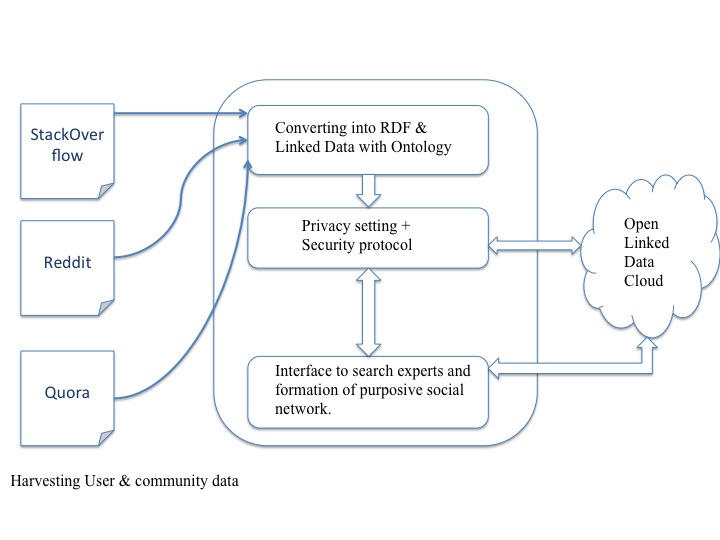
\includegraphics[width=15cm]{Slide2.jpg}
  \caption{System design and framework for the formation of purposive social network using Linked Data}
  \label{Figure:figex5a}
\end{figure}

\subsection{Gantt chart}

The \fref{Figure:figex5b} of  Gantt chart outlines the timeline and the tasks required for the next ten months (40 weeks) to complete my thesis. Below it is a proposal to create a prototype of the system that harvest the online user and community data from Reddit and Quora, convert it into Linked Data and link it to the Linked Data Cloud.  The system will also provide a user interface to browse and search the linked data so users can find right people with appropriate expertise to form purposive community and interact with each other.

\begin{figure}[!htb]
  \centering
  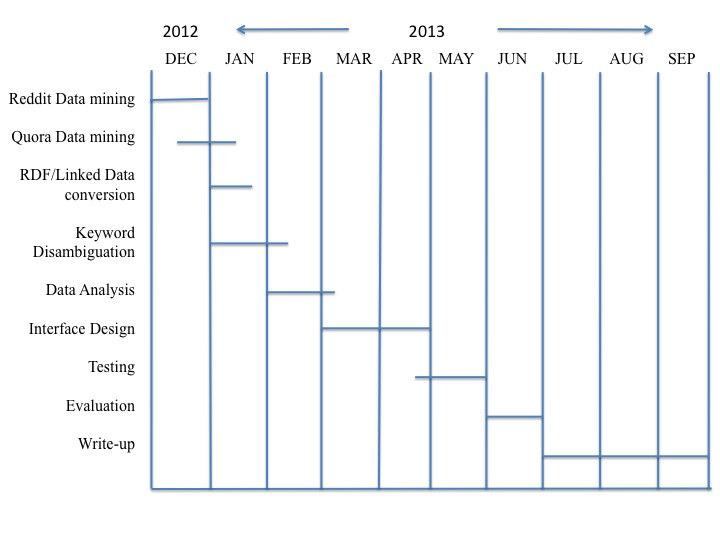
\includegraphics[width=15cm]{Slide1.jpg}
  \caption{Gantt chart showing the timeline of task to do for writing PhD thesis}
  \label{Figure:figex5b}
\end{figure}

The tasks to implement the prototype of the framework are as follows:

\subsubsection{Reddit Data mining (Week 1-4)}

The first month will be used mine the Reddit website data, especially from the programming sub-reddits. This will include the questions asked, users comments with the up votes and down votes of each post. The user profile information will also be collected to create a knowledgebase of experts in a field.

\subsubsection{Quora Data mining (Week 3-6)}

The data from Quora website can be simultaneously harvested with the Reddit data as it requires the same program with slight alteration of code. The programming categories will be used to gather questions and answers with the votes and user information.

\subsubsection{RDF/Linked Data conversion (Week 5-7)}

The program that converted StackOverflow data can reuse the same ontology to convert the Reddit and Quora data into RDF and Linked Data. The program can run in the background so when the Reddit and Quora data is being harvested, it will also be converted into RDF and N-Triples and saved in a Triplestore.

\subsubsection{Keyword disambiguation (Week 4-10)}

As the previous task, WIkipedia miner program and OpenCalis web service can run in the background and simultaneously get the website posts, use the web service to do natural language processing, find the main topics and keywords and link it to the appropriate Wikipedia topic and Drupal vocabulary. This phase will also include linking the data to the Open Linked Data Cloud and creating a integrated knowledgebase.

\subsubsection{Data Analysis (Week 9-13)}

This task requires analysing the Linked Data, RDF and keywords data to find the main topics, remove the noise and find the best sample set to perform the final analysis to prove the concept of purposive social network and using the linked data to improve search and discovery of expert.

\subsubsection{Interface Design (Week 13-20)}

The main developments of the front end, the algorithm to query and search the user data and community data, the design of user interface and the final deployment of the framework will be done in the span of two month. A simple user interface will be designed so people can search for experts on any topic and also search for information from the integrated knowledgebase of the three website used in the experiments.

\subsubsection{Testing (Week 19-24)}

The final week of programming will coincide with the first week of testing of the system and the next three week will be utilized in fixing the bugs in any of the features and design.

\subsubsection{Evaluation (Week 25-28)}

Once the testing is finished and the system is working properly, the system shall be evaluated. It could be a user evaluation or statistical evaluation and the generated data is analyzed to gather the final result.

\subsubsection{Thesis write-up (Week 29-40)}

The last three month will be used for writing the thesis incorporating all the procedures, algorithms and results generated from the system. The literature currently read and review will be included with addition literature reviewed in the mean time.